\secrel{Введение в KiCAD}\secdown

Подробно пакет \prog{KiCAD}\ рассмотрен в разделе \ref{kicad}. В этом разделе
очень кратко продублирован минимум информации об этой программе\note{САПР
электронных устройств, EDA CAD}, чтобы вы легко и быстро смогли начать
разрабатывать печатные платы для своих простых поделок. В оригинальной книге
\cite{bcollis}\ рассматривается пакет \prog{Eagle}, но бесплатная лицензия на
\prog{Eagle} запрещает использовать ее для коммерческих проектов, и размер плат
ограничен до 100\,мм $\times$ 80\,мм, поэтому была сделана замена САПР. EDA САПР
позволяет пользователю рисовать схемы для электронных цепей, и затем на их
основе \termdef{трассиров\'{а}ть}{трассир\'{о}вка печатной платы} печатные
платы. Используя этот очень краткий пошаговый учебник, вы
\termdef{развед\'{е}те}{разв\'{о}дка печатной платы} плату для схемы усилителя
на микросхеме TDA2822.

\secrel{Менеджер проектов \prog{kicad}}

\win: \menu{\winstart>Программы>KiCAD>KiCAD}

\linux: \verb|user@host$ kicad|

\bigskip
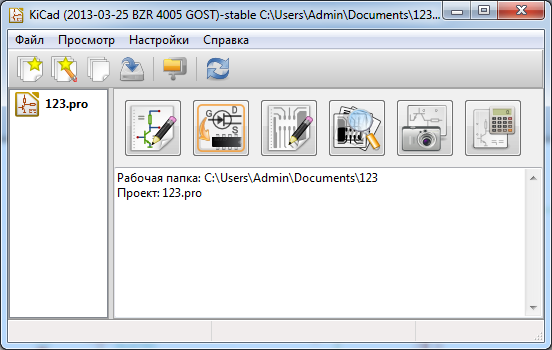
\includegraphics[height=0.8\textheight]{kicad/projman.png}

\bigskip
В верхней части панели \term{менеджера проектов} \prog{kicad} имеются большие
кнопки запуска компонентов KiCad:

\begin{itemize}
\item
\includegraphics[height=0.1\textheight]{tmp/icon_eeschema.png}
\prog{eeschema}\ --- Редактор принципиальных схем
\item

\includegraphics[height=0.1\textheight]{kicad/icon_pcbnew.png}
\prog{pcbnew}\ --- Редактор печатных плат
\item
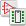
\includegraphics[height=0.1\textheight]{kicad/icon_cvpcb.png}
\prog{cvpcb}\ --- Программа редактирования \termdef{падстеков}{падстек}
(отверстий и площадок)
\end{itemize}

Каждая кнопка запускает соответствующую программу. Мы будем использовать эти
программы по мере изучения.


\secrel{Создание схемы в модуле \eeschema}


Запустите из менеджера проектов, графической оболочки или командной строки
\linux\ модуль \eeschema: 

\bigskip
\noindent\verb|user@host$ eeschema &|.

\bigskip
\noindent\includegraphics[height=0.1\textheight]{kicad/icon_eeschema.png}

\clearpage\noindent
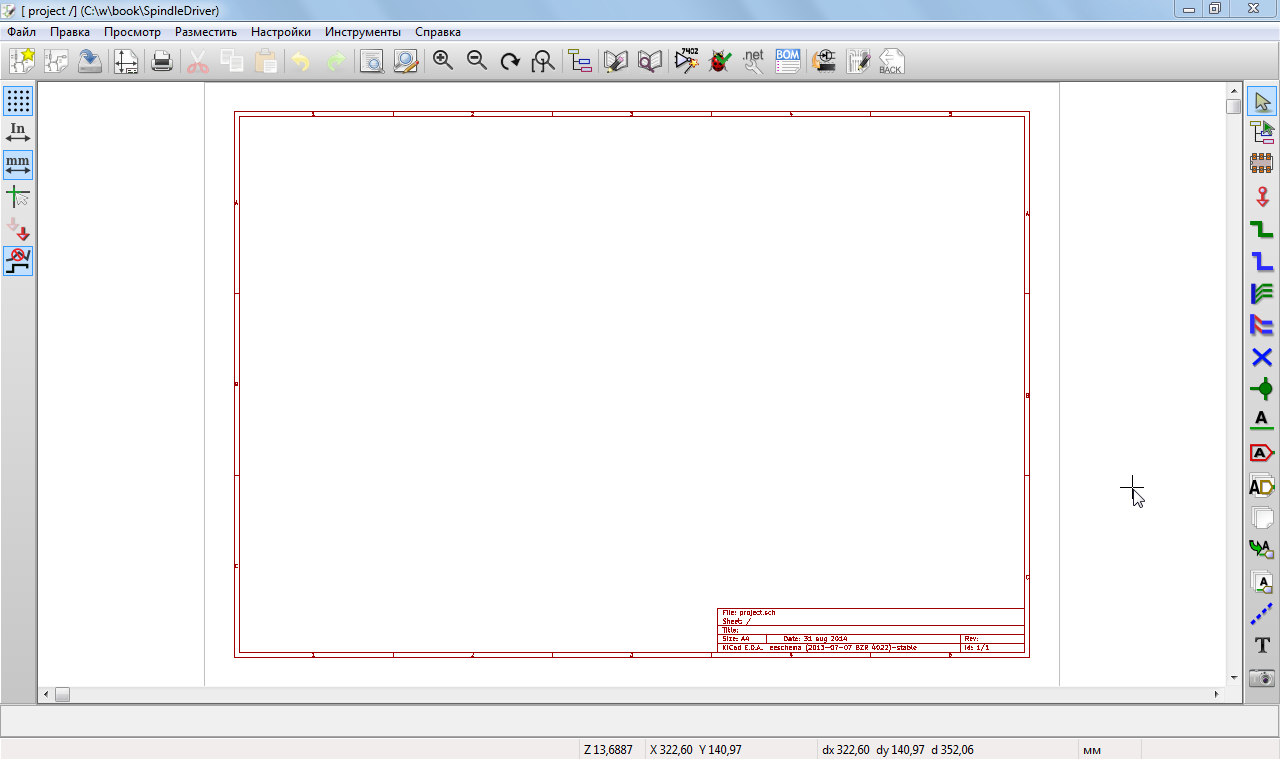
\includegraphics[width=\textwidth]{kicad/ee15.png}

На правом краю окна редактора схем есть вертикальная панель инструментов,
которые мы и будем использовать для рисования схемы. Этими инструментами можно
выбирать объекты, размещать компоненты, вводить связи и т.д.


\secrel{Сохранение схемы}

\begin{itemize}
  \item 
Не забывайте сохранять ваши данные в процессе работы
  \item 
САПР создает много временных файлов, так что вы должны держать ваши папки в
аккуратности.
  \item 
Если в первый раз запустили \prog{eeschema}, создайте папку для проекта.
  \item 
Создайте папку в соответствии с названием проекта, например, \file{DarkDetector}
  \item 
Сохраните схему как \file{DarkDetector.sch} в папке \file{DarkDetector}.
\end{itemize}

\secup
